\clearpage
\VerdierPhysicalPageAnchor{0093}%
\begingroup
\setlength{\abovedisplayskip}{5pt plus 2pt minus 2pt}%
\setlength{\belowdisplayskip}{5pt plus 2pt minus 2pt}%
\VerdierSemanticAnchor{ch1-3-2-10-qpf-functorial-map}
同样，态射 $q(p(f))\colon c(p(f))\longrightarrow Y[1]$
表示函子态射：

\VerdierSemanticAnchor{ch1-3-2-10-eq3}
\begin{equation}
  \begin{gathered}
    D=
    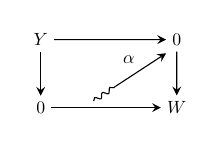
\begin{tikzpicture}[>=stealth,baseline=(current bounding box.center),scale=0.64,
      every node/.style={transform shape}]
      \node (Y) at (0,1.35) {$Y$};
      \node (ZT) at (2.7,1.35) {$0$};
      \node (ZB) at (0,0) {$0$};
      \node (W) at (2.7,0) {$W$};
      \draw[->] (Y) -- (ZT); \draw[->] (Y) -- (ZB);
      \draw[->] (ZT) -- (W); \draw[->] (ZB) -- (W);
      \draw[decorate,decoration={snake,amplitude=0.8pt,segment length=3.3pt}]
        (1.05,0.13) -- (1.48,0.42);
      \draw[->] (1.48,0.42) -- node[above left] {$\alpha$} (2.49,1.08);
    \end{tikzpicture}
    \quad\longmapsto\quad
    q(p(f))D=
    \bigl(0\colon Y\longrightarrow W,\;
      \alpha\colon0\rightsquigarrow0,\;
      0\colon0\rightsquigarrow0\bigr).
  \end{gathered}
  \tag{3.2.10.3}
\end{equation}

\VerdierSemanticAnchor{ch1-3-2-10-conclusion}
因此，利用 (3.2.8.4)，为证明 (3.2.7.4)，只需注意，对每个图
\[
  D=
  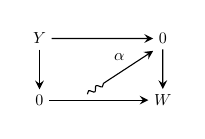
\begin{tikzpicture}[>=stealth,baseline=(current bounding box.center),scale=0.58,
    every node/.style={transform shape}]
    \node (Y) at (0,1.35) {$Y$};
    \node (ZT) at (2.7,1.35) {$0$};
    \node (ZB) at (0,0) {$0$};
    \node (W) at (2.7,0) {$W$};
    \draw[->] (Y) -- (ZT); \draw[->] (Y) -- (ZB);
    \draw[->] (ZT) -- (W); \draw[->] (ZB) -- (W);
    \draw[decorate,decoration={snake,amplitude=0.8pt,segment length=3.3pt}]
      (1.05,0.13) -- (1.48,0.42);
    \draw[->] (1.48,0.42) -- node[above left] {$\alpha$} (2.49,1.08);
  \end{tikzpicture}
  \qquad Hq(p(f))D+f[1]D=0.
\]

\VerdierSemanticAnchor{ch1-3-2-11}
\noindent\textbf{3.2.11.}
\VerdierSemanticAnchor{ch1-3-2-11-composable-morphisms}
设 $X\xrightarrow{f}Y\xrightarrow{g}Z$ 是 $\operatorname{comp}(C)$ 中
两个态射。置 $gf=h$。利用这些数据，可以构造两个交换图：

\VerdierSemanticAnchor{ch1-3-2-11-eq1}
\begin{equation}
  \begin{gathered}
  D=
  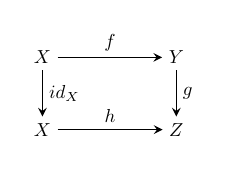
\begin{tikzpicture}[>=stealth,baseline=(current bounding box.center),scale=0.68,
    every node/.style={transform shape}]
    \node (X1) at (0,1.35) {$X$}; \node (Y) at (2.5,1.35) {$Y$};
    \node (X2) at (0,0) {$X$}; \node (Z) at (2.5,0) {$Z$};
    \draw[->] (X1) -- node[above] {$f$} (Y);
    \draw[->] (X1) -- node[right] {$\operatorname{id}_X$} (X2);
    \draw[->] (Y) -- node[right] {$g$} (Z);
    \draw[->] (X2) -- node[above] {$h$} (Z);
  \end{tikzpicture},
  \qquad
  D'=
  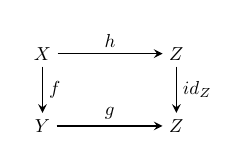
\begin{tikzpicture}[>=stealth,baseline=(current bounding box.center),scale=0.68,
    every node/.style={transform shape}]
    \node (X) at (0,1.35) {$X$}; \node (Z1) at (2.5,1.35) {$Z$};
    \node (Y) at (0,0) {$Y$}; \node (Z2) at (2.5,0) {$Z$};
    \draw[->] (X) -- node[above] {$h$} (Z1);
    \draw[->] (X) -- node[right] {$f$} (Y);
    \draw[->] (Z1) -- node[right] {$\operatorname{id}_Z$} (Z2);
    \draw[->] (Y) -- node[above] {$g$} (Z2);
  \end{tikzpicture}
  \end{gathered}
  \tag{3.2.11.1}
\end{equation}

\VerdierSemanticAnchor{ch1-3-2-11-cone-images}
我们把它们解释为 $\operatorname{tr}_1(C)$ 的态射。因此，应用映射锥函子，
得到两个图：
\[
  c(f)\xrightarrow{c(D)}c(h)\xrightarrow{c(D')}c(g)
\]

\VerdierSemanticAnchor{ch1-3-2-11-eq2}
\begin{equation}
  I=
  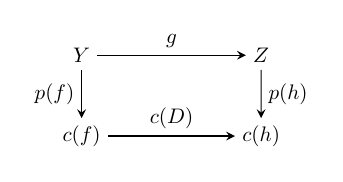
\begin{tikzpicture}[>=stealth,baseline=(current bounding box.center),scale=0.76,
    every node/.style={transform shape}]
    \node (Y) at (0,1.35) {$Y$}; \node (Z) at (3.0,1.35) {$Z$};
    \node (Cf) at (0,0) {$c(f)$}; \node (Ch) at (3.0,0) {$c(h)$};
    \draw[->] (Y) -- node[above] {$g$} (Z);
    \draw[->] (Y) -- node[left] {$p(f)$} (Cf);
    \draw[->] (Z) -- node[right] {$p(h)$} (Ch);
    \draw[->] (Cf) -- node[above] {$c(D)$} (Ch);
  \end{tikzpicture}
  \tag{3.2.11.2}
\end{equation}

\VerdierSemanticAnchor{ch1-3-2-11-ci-morphism}
最后这个图是一个交换方形 (3.2.2.4)，因而可以解释为
$\operatorname{tr}_1(C)$ 的一个态射。再次应用映射锥函子，得到态射：

\VerdierSemanticAnchor{ch1-3-2-11-eq3}
\begin{equation}
  c(I)\colon c(g)\longrightarrow c(c(D)).
  \tag{3.2.11.3}
\end{equation}
\endgroup
